\chapter{Theoretical framework}

\section{Phase-locked loop fundamentals}
\subsection{Basic structure}
\subsection{Key PLL parameters}
\subsubsection{Phase noise / jitter}
Jitter is defined as the time deviation ($\Delta_t$) of a signal's transition edges from their ideal positions in time. It is a metric of the outmost importance in the design of PLLs 
as it is a direct measure of the quality of the clock signal generated. Phase noise describes the same phenomenon in the frequency domain (the phase noise of a signal is the Fourier 
transform of the jitter) and is usually expressed in dBc/Hz.
\subsubsection{Output frequency}
It is defined as the range of frequencies that the PLL is capable of generating and can be determined by the VCO output range and the division ratio of the feedback frequency divider. This
is a key metric in establishing the application of the PLL (e.g., clock generation or RF synthesizer) and it bears significant importance in the design process due to the tradeoff 
it has with the phase noise performance of the PLL.
\subsubsection{Loop bandwidth}
The closed-loop bandwidth of a PLL is the frequency range over which the PLL can track the phase/frequency variations of the input signal (from DC to -3 dB from the open-loop 
gain). It affects the acquisition time and phase noise performance of the PLL.
\subsubsection{Noise bandwidth}
It is the PLL's noise due to the filter's loop bandwidth, the higher frequencies of the voltage-controlled oscillator (VCO) are the major
contributor to this effect, therefore the need to set a low enough bandwidth in order to supress the most out of it. Even if reducing the loop
bandwidth would be desirable to supress in-band phase noise, it's also necessary to take into consideration that there is a tradeoff between the
lock-in time and in-band phase noise.
\subsubsection{Beat-note period}
Defined as the time interval between successive "beats" (oscillations) observed at the phase detector output, in other words, is the inverse of
the frequency difference's magnitude between the reference and feedback signals as shown in figure \ref{fig:PFD_output}. Beat-note period is closely related to the acquisition time of the
PLL and can be estimated by equation \eqref{eq:T_beat}. 

\begin{equation}
    T_{beat} = \frac{1}{|f_{ref} - f_{feed}|}
    \label{eq:T_beat}
\end{equation}


\begin{minipage}{0.35\textwidth}
    \begin{center}
        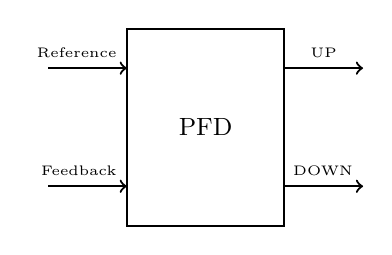
\begin{tikzpicture}
            \draw[->, thick] (-1,2) -- (0,2) node[anchor=south east] {\tiny Reference};
            \draw[->, thick] (-1, 0.5) -- (0,0.5) node[anchor=south east] {\tiny Feedback};
            \draw[thick] (0,0) rectangle (2,2.5);   %PFD
            \draw node at (1,1.25) {\small PFD};
            \draw[->, thick] (2,0.5) -- (3,0.5) node[anchor=south east] {\tiny DOWN};
            \draw[->, thick] (2,2) -- (3,2);
            \draw node at (2.5,2.2) {\tiny UP};
        \end{tikzpicture}
        \captionof{figure}{a) PFD block.}
        \label{fig:PFD_block}
    \end{center}
\end{minipage}
\hspace{0.13\textwidth}
\begin{minipage}{0.5\textwidth}
    \begin{center}
        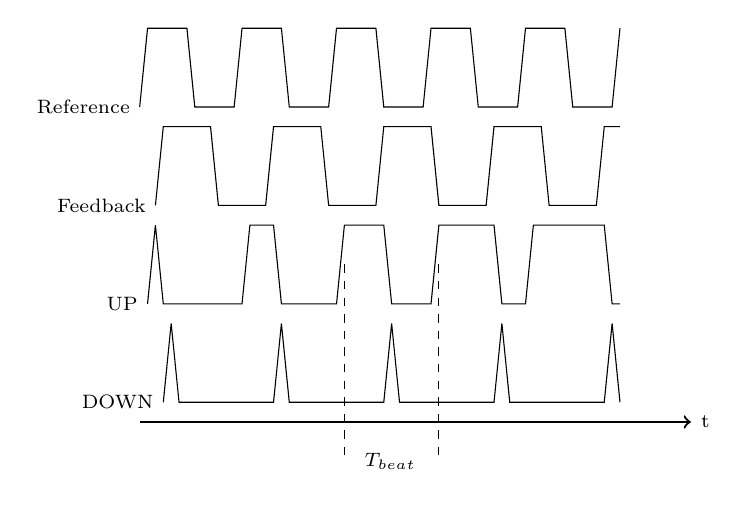
\begin{tikzpicture}
            \draw[->, thick] (0,1) -- (7,1) node[anchor=west] {\scriptsize t};
            \draw (0,5) node[anchor=east] {\scriptsize Reference} -- (0.1,6) -- (0.6,6) -- (0.7,5) -- (1.2,5) -- (1.3,6) -- (1.8,6) -- (1.9,5) -- (2.4,5) -- (2.5,6) -- (3,6) -- (3.1,5) -- (3.6,5) -- (3.7,6) -- (4.2,6) -- (4.3,5) -- (4.8,5) -- (4.9,6) -- (5.4,6) -- (5.5,5) -- (6,5) -- (6.1,6);
            \draw (0.2,3.75) node[anchor=east] {\scriptsize Feedback} -- (0.3,4.75) -- (0.9,4.75) -- (1,3.75) -- (1.6,3.75) -- (1.7,4.75) -- (2.3,4.75) -- (2.4,3.75) -- (3,3.75) -- (3.1,4.75) -- (3.7,4.75) -- (3.8,3.75) -- (4.4,3.75) -- (4.5,4.75) -- (5.1,4.75) -- (5.2,3.75) -- (5.8,3.75) -- (5.9,4.75) -- (6.1,4.75);
            \draw (0.1,2.5) node[anchor=east] {\scriptsize UP} -- (0.2,3.5) -- (0.3,2.5) -- (1.3,2.5) -- (1.4,3.5) -- (1.7,3.5) -- (1.8,2.5) -- (2.5,2.5) -- (2.6,3.5) -- (3.1,3.5) -- (3.2,2.5) -- (3.7,2.5) -- (3.8,3.5) -- (4.5,3.5) -- (4.6,2.5) -- (4.9,2.5) -- (5,3.5) -- (5.9,3.5) -- (6,2.5) -- (6.1,2.5);
            \draw (0.3,1.25) node[anchor=east] {\scriptsize DOWN} -- (0.4,2.25) -- (0.5,1.25) -- (1.7,1.25) -- (1.8,2.25) -- (1.9,1.25) -- (3.1,1.25) -- (3.2,2.25) -- (3.3,1.25) -- (4.5,1.25) -- (4.6,2.25) -- (4.7,1.25) -- (5.9,1.25) -- (6,2.25) -- (6.1,1.25);
            \draw[dashed] (2.6,3) -- (2.6,0.5) node[right, outer sep=4pt] {\scriptsize $T_{beat}$};
            \draw[dashed] (3.8,3) -- (3.8,0.5);
        \end{tikzpicture}
        \captionof{figure}{b) PFD output.}
        \label{fig:PFD_output}
    \end{center}
\end{minipage}
\subsubsection{Lock-in time}
Lock-in time (also called aquisition time) is defined as the time for the PLL to lock onto the input reference phase and frequency within one 
beat-note period after a frequency change or startup of the system. It is a fast locking process.
\subsubsection{Pull-in time}
danan
\subsubsection{Lock-in range}
adnna
\subsubsection{Pull-in range}
anan
\subsubsection{Pull-out range}
nana
\subsubsection{Hold range}
fdan
\subsubsection{SNR}
adfn
\subsubsection{Power consumption}
dfanna
\subsubsection{Spurious tones}
fdafdhdhdah

\subsection{Analog phase-locked loops}
dfanadn
\subsection{Linearized model}
daan
\subsection{Digital phase-locked loops}
anan
\section{Time-to-digital converters}
\subsection{Delay-locked loop fundamentals}
\subsection{TDC as a phase detector}

\section{65 nm CMOS technology}
